\documentclass{article}\usepackage[]{graphicx}\usepackage[]{color}
%% maxwidth is the original width if it is less than linewidth
%% otherwise use linewidth (to make sure the graphics do not exceed the margin)
\makeatletter
\def\maxwidth{ %
  \ifdim\Gin@nat@width>\linewidth
    \linewidth
  \else
    \Gin@nat@width
  \fi
}
\makeatother

\definecolor{fgcolor}{rgb}{0.345, 0.345, 0.345}
\newcommand{\hlnum}[1]{\textcolor[rgb]{0.686,0.059,0.569}{#1}}%
\newcommand{\hlstr}[1]{\textcolor[rgb]{0.192,0.494,0.8}{#1}}%
\newcommand{\hlcom}[1]{\textcolor[rgb]{0.678,0.584,0.686}{\textit{#1}}}%
\newcommand{\hlopt}[1]{\textcolor[rgb]{0,0,0}{#1}}%
\newcommand{\hlstd}[1]{\textcolor[rgb]{0.345,0.345,0.345}{#1}}%
\newcommand{\hlkwa}[1]{\textcolor[rgb]{0.161,0.373,0.58}{\textbf{#1}}}%
\newcommand{\hlkwb}[1]{\textcolor[rgb]{0.69,0.353,0.396}{#1}}%
\newcommand{\hlkwc}[1]{\textcolor[rgb]{0.333,0.667,0.333}{#1}}%
\newcommand{\hlkwd}[1]{\textcolor[rgb]{0.737,0.353,0.396}{\textbf{#1}}}%

\usepackage{framed}
\makeatletter
\newenvironment{kframe}{%
 \def\at@end@of@kframe{}%
 \ifinner\ifhmode%
  \def\at@end@of@kframe{\end{minipage}}%
  \begin{minipage}{\columnwidth}%
 \fi\fi%
 \def\FrameCommand##1{\hskip\@totalleftmargin \hskip-\fboxsep
 \colorbox{shadecolor}{##1}\hskip-\fboxsep
     % There is no \\@totalrightmargin, so:
     \hskip-\linewidth \hskip-\@totalleftmargin \hskip\columnwidth}%
 \MakeFramed {\advance\hsize-\width
   \@totalleftmargin\z@ \linewidth\hsize
   \@setminipage}}%
 {\par\unskip\endMakeFramed%
 \at@end@of@kframe}
\makeatother

\definecolor{shadecolor}{rgb}{.97, .97, .97}
\definecolor{messagecolor}{rgb}{0, 0, 0}
\definecolor{warningcolor}{rgb}{1, 0, 1}
\definecolor{errorcolor}{rgb}{1, 0, 0}
\newenvironment{knitrout}{}{} % an empty environment to be redefined in TeX

\usepackage{alltt}

\usepackage{booktabs}
\usepackage[top=2.5cm, bottom=2.5cm, left=2.5cm, right=2.5cm]{geometry}
\usepackage{wasysym}

\usepackage{float}
\usepackage{tikz} % for arrows and figures
\usetikzlibrary{positioning,decorations.pathreplacing,shapes}

\title{Can we "infer" causality with a single linear model in the case of a non-linear causal path?}
\date{\today} %%If commented, the current date is used.

\author{Timoth\'{e}e Bonnet}
\IfFileExists{upquote.sty}{\usepackage{upquote}}{}
\begin{document}

\maketitle

After the talk of this pervert mouse rapist, we were wondering whether a linear model is enough to identify correctly causality when there are direct and indirect effects of a cause. 


Let's figure this out, by first creating some data using this function:

\begin{knitrout}
\definecolor{shadecolor}{rgb}{0.969, 0.969, 0.969}\color{fgcolor}\begin{kframe}
\begin{alltt}
\hlstd{fiat_datum}\hlkwb{<-}\hlkwa{function}\hlstd{(}\hlkwc{AB}\hlstd{=}\hlnum{3}\hlstd{,}\hlkwc{BC}\hlstd{=}\hlnum{4}\hlstd{,}\hlkwc{AC}\hlstd{=}\hlnum{2}\hlstd{,}\hlkwc{nbpt}\hlstd{=}\hlnum{1000}\hlstd{,}\hlkwc{noise}\hlstd{=}\hlnum{0}\hlstd{,} \hlkwc{nastiness}\hlstd{=}\hlnum{0}\hlstd{)}
\hlstd{\{}
\hlstd{unobservedProcess1}\hlkwb{<-}\hlkwd{runif}\hlstd{(}\hlkwc{n}\hlstd{=nbpt,}\hlkwc{min} \hlstd{=} \hlopt{-}\hlnum{1}\hlstd{,}\hlkwc{max}\hlstd{=}\hlnum{1}\hlstd{)}
\hlstd{unobservedProcess2}\hlkwb{<-}\hlkwd{runif}\hlstd{(}\hlkwc{n}\hlstd{=nbpt,}\hlkwc{min} \hlstd{=} \hlopt{-}\hlnum{1}\hlstd{,}\hlkwc{max}\hlstd{=}\hlnum{1}\hlstd{)}
\hlstd{cause}\hlkwb{<-}\hlkwd{rnorm}\hlstd{(}\hlkwc{n} \hlstd{= nbpt,}\hlkwc{mean}\hlstd{=}\hlnum{1}\hlstd{,}\hlkwc{sd}\hlstd{=}\hlnum{3}\hlstd{)}
\hlstd{consequence1}\hlkwb{<-}\hlstd{(}\hlnum{5}\hlopt{+}\hlstd{cause}\hlopt{*}\hlstd{AB}\hlopt{+}\hlkwd{rnorm}\hlstd{(nbpt,}\hlkwc{mean}\hlstd{=}\hlnum{0}\hlstd{,}\hlkwc{sd} \hlstd{=} \hlnum{2}\hlstd{)}\hlopt{-}\hlstd{noise}\hlopt{*}\hlnum{1.5}\hlopt{*}\hlstd{unobservedProcess1)}\hlopt{^}\hlstd{(}\hlnum{1}\hlopt{+}\hlstd{nastiness)}
\hlstd{consequence2}\hlkwb{<-}\hlnum{2}\hlopt{+}\hlstd{cause}\hlopt{*}\hlstd{AC}\hlopt{+}\hlstd{consequence1}\hlopt{*}\hlstd{BC}\hlopt{+}\hlkwd{rnorm}\hlstd{(nbpt,}\hlkwc{mean}\hlstd{=}\hlnum{0}\hlstd{,}\hlkwc{sd}\hlstd{=}\hlnum{2}\hlstd{)}\hlopt{+}\hlstd{noise}\hlopt{*}\hlnum{10}\hlopt{*}\hlstd{unobservedProcess2}

\hlstd{df}\hlkwb{<-}\hlkwd{data.frame}\hlstd{(cause, consequence1,consequence2)}
\hlstd{\}}

\hlstd{df}\hlkwb{<-}\hlkwd{fiat_datum}\hlstd{()}
\end{alltt}
\end{kframe}
\end{knitrout}

When we keep it very simple, it looks like this:
\begin{knitrout}
\definecolor{shadecolor}{rgb}{0.969, 0.969, 0.969}\color{fgcolor}

{\centering 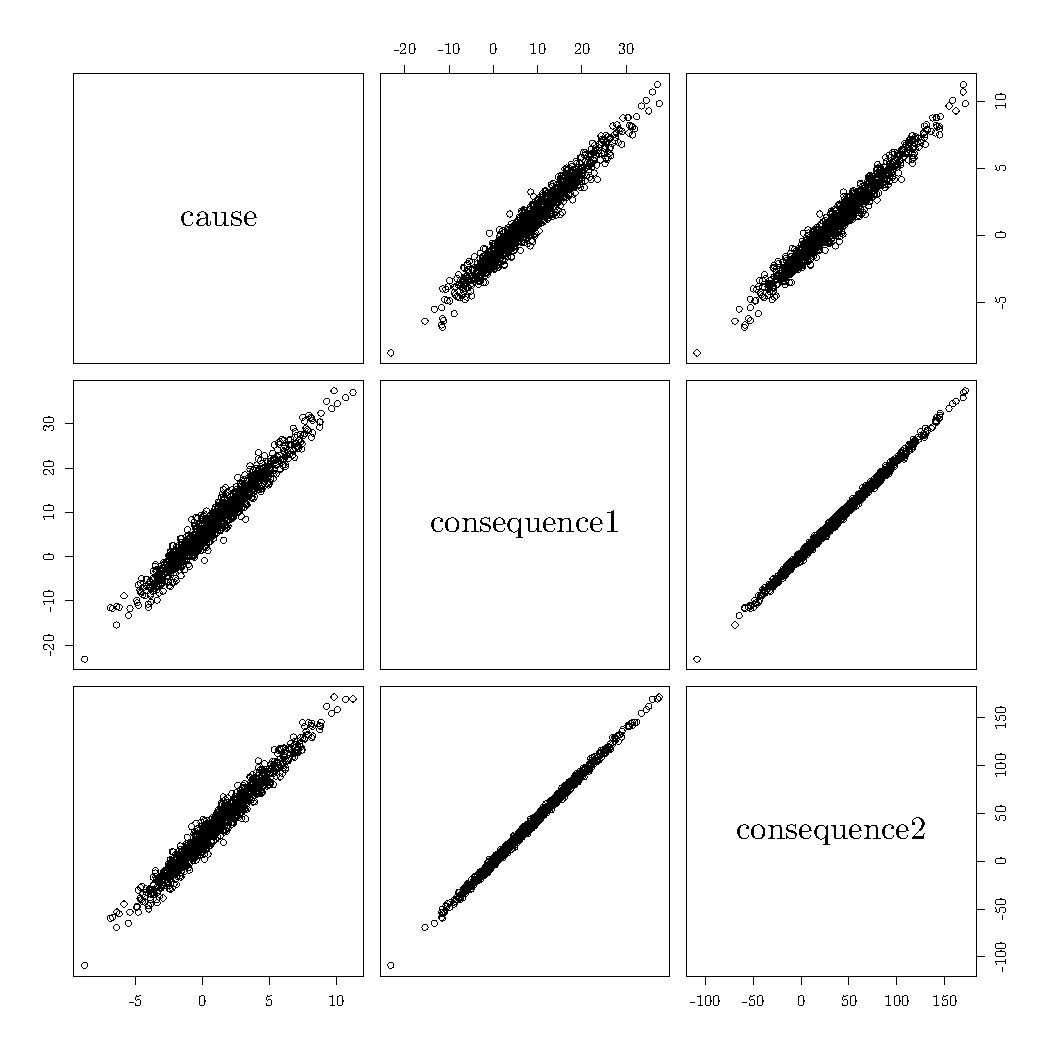
\includegraphics[width=0.6\textwidth]{figure/ShowData-1} 

}



\end{knitrout}

The idea behind it, is that a cause A affects a variable B and a variable C, while B also affects C. 


\begin{figure}[H]
\centering
\label{figure:causal}
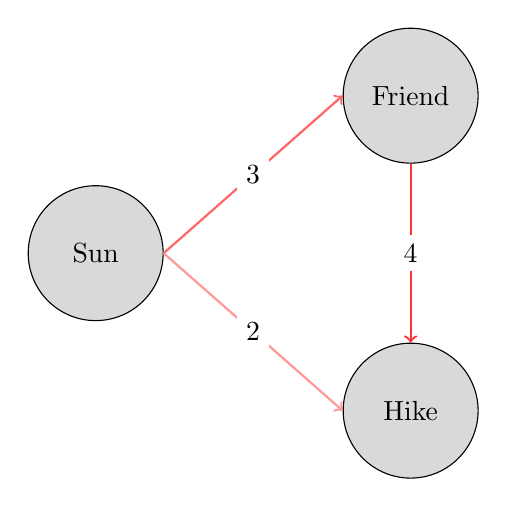
\begin{tikzpicture}[%
  % common options for blocks:
  block/.style = {draw, fill=blue!30, align=center, anchor=north,
              minimum height=0.55cm, inner sep=0},
  % common options for the circles:
  ball/.style = {circle, draw, align=center, anchor=north, inner sep=0}
	]
  
  \node[ball, fill=gray!30,text width=1.7cm] (A) at (0,0) {Sun};
  \node[ball, fill=gray!30,text width=1.7cm] (B) at (4,2) {Friend};
  \node[ball, fill=gray!30,text width=1.7cm] (C) at (4,-2) {Hike};

  \draw[->,thick,draw=red!60] (A.east) -- (B.west)
  node[midway,fill=white] (midway) {3};
  \draw[->,thick,draw=red!40] (A.east) -- (C.west)
    node[midway,fill=white] (midway) {2};
  \draw[->,thick,draw=red!80] (B.south) -- (C.north)
    node[midway,fill=white] (midway) {4};
\end{tikzpicture}
\caption{Causal path between the possibility to go hiking during the weekend, the weather, and a lovely friend going hiking. The arrows indicate the direction of causality. Their color and the number in their middle indicates the slope beween the variables.}
\end{figure}


Can we find back the causal coefficients Sun $\rightarrow$ Hike and Friend $\rightarrow$ Hike, using only a multiple regression?


\begin{knitrout}
\definecolor{shadecolor}{rgb}{0.969, 0.969, 0.969}\color{fgcolor}\begin{kframe}
\begin{alltt}
\hlstd{m0}\hlkwb{<-}\hlkwd{lm}\hlstd{(consequence2}\hlopt{~}\hlnum{1}\hlopt{+}\hlstd{cause}\hlopt{+}\hlstd{consequence1,}\hlkwc{data}\hlstd{=df)}
\hlkwd{summary}\hlstd{(m0)}
\end{alltt}
\begin{verbatim}
## 
## Call:
## lm(formula = consequence2 ~ 1 + cause + consequence1, data = df)
## 
## Residuals:
##    Min     1Q Median     3Q    Max 
## -6.597 -1.331 -0.050  1.362  6.336 
## 
## Coefficients:
##              Estimate Std. Error t value Pr(>|t|)    
## (Intercept)   2.28725    0.17783   12.86   <2e-16 ***
## cause         2.05100    0.09851   20.82   <2e-16 ***
## consequence1  3.96755    0.03231  122.78   <2e-16 ***
## ---
## Signif. codes:  0 '***' 0.001 '**' 0.01 '*' 0.05 '.' 0.1 ' ' 1
## 
## Residual standard error: 1.992 on 997 degrees of freedom
## Multiple R-squared:  0.9979,	Adjusted R-squared:  0.9978 
## F-statistic: 2.316e+05 on 2 and 997 DF,  p-value: < 2.2e-16
\end{verbatim}
\end{kframe}
\end{knitrout}

Yes, the two independent variables do control one each other, the estimation is not biased. However, maybe the accuracy of the estimation is affected by the correlation between them.

Let's generate data with a stronger dependency between the cause and the first consequence, keeping the other two causal path constants.

\begin{knitrout}
\definecolor{shadecolor}{rgb}{0.969, 0.969, 0.969}\color{fgcolor}\begin{kframe}
\begin{alltt}
\hlstd{df2}\hlkwb{<-}\hlkwd{fiat_datum}\hlstd{(}\hlkwc{AB}\hlstd{=}\hlnum{8}\hlstd{)}
\hlkwd{plot}\hlstd{(df2)}
\end{alltt}
\end{kframe}

{\centering 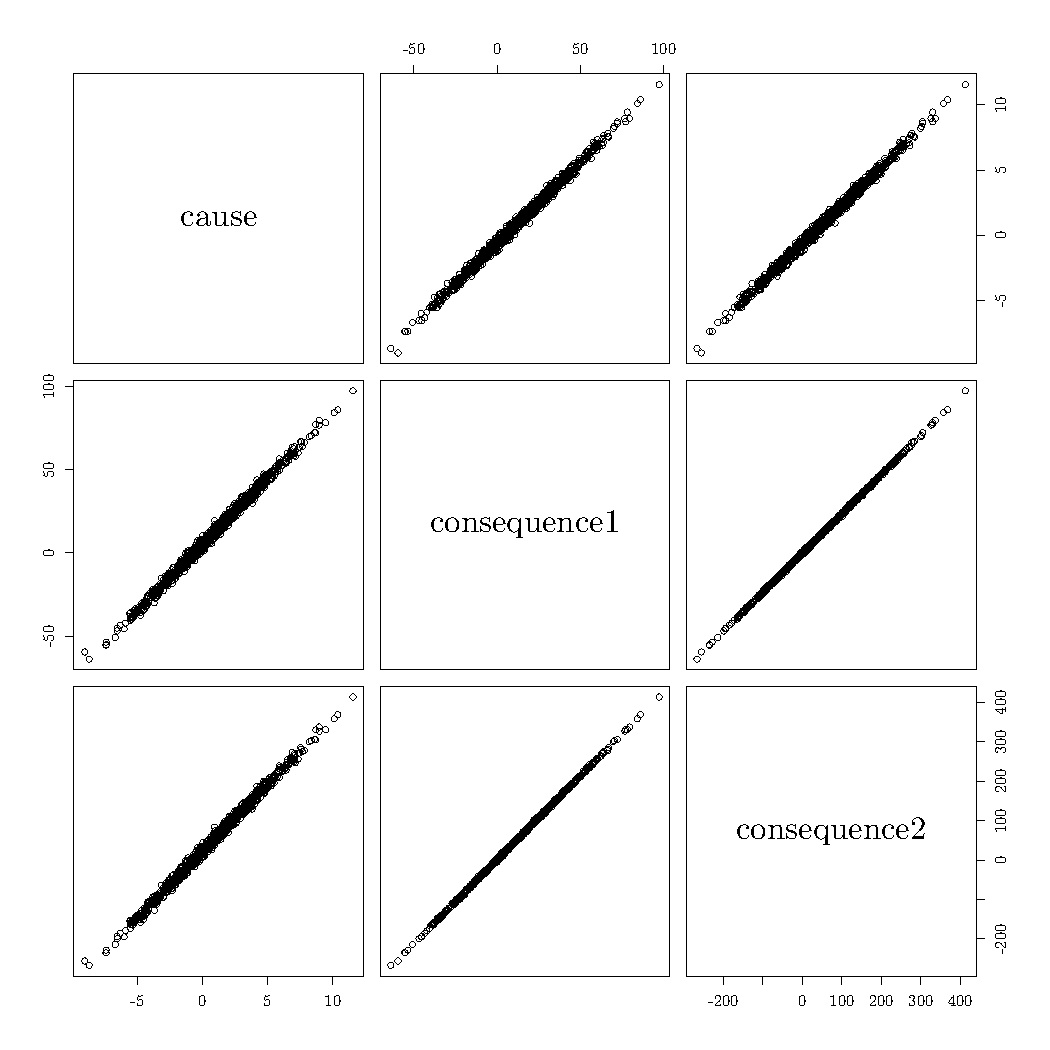
\includegraphics[width=0.6\textwidth]{figure/dataCor-1} 

}



\end{knitrout}

\begin{knitrout}
\definecolor{shadecolor}{rgb}{0.969, 0.969, 0.969}\color{fgcolor}\begin{kframe}
\begin{alltt}
\hlstd{m1}\hlkwb{<-}\hlkwd{lm}\hlstd{(consequence2}\hlopt{~}\hlnum{1}\hlopt{+}\hlstd{cause}\hlopt{+}\hlstd{consequence1,}\hlkwc{data}\hlstd{=df2)}
\hlkwd{summary}\hlstd{(m1)}
\end{alltt}
\begin{verbatim}
## 
## Call:
## lm(formula = consequence2 ~ 1 + cause + consequence1, data = df2)
## 
## Residuals:
##     Min      1Q  Median      3Q     Max 
## -6.3074 -1.3492 -0.0112  1.4763  6.9590 
## 
## Coefficients:
##              Estimate Std. Error t value Pr(>|t|)    
## (Intercept)   2.23758    0.17646   12.68   <2e-16 ***
## cause         2.36869    0.26173    9.05   <2e-16 ***
## consequence1  3.95427    0.03274  120.79   <2e-16 ***
## ---
## Signif. codes:  0 '***' 0.001 '**' 0.01 '*' 0.05 '.' 0.1 ' ' 1
## 
## Residual standard error: 2.006 on 997 degrees of freedom
## Multiple R-squared:  0.9996,	Adjusted R-squared:  0.9996 
## F-statistic: 1.371e+06 on 2 and 997 DF,  p-value: < 2.2e-16
\end{verbatim}
\end{kframe}
\end{knitrout}

The estimate does not seem biased, let's check it seriously:
\begin{knitrout}
\definecolor{shadecolor}{rgb}{0.969, 0.969, 0.969}\color{fgcolor}\begin{kframe}
\begin{alltt}
\hlstd{vectcause}\hlkwb{<-}\hlkwd{replicate}\hlstd{(}\hlkwc{n} \hlstd{=} \hlnum{1000}\hlstd{,}\hlkwc{expr} \hlstd{= \{}\hlkwd{lm}\hlstd{(consequence2}\hlopt{~}\hlnum{1}\hlopt{+}\hlstd{cause}\hlopt{+}\hlstd{consequence1,}
                                         \hlkwc{data}\hlstd{=}\hlkwd{fiat_datum}\hlstd{(}\hlkwc{AB}\hlstd{=}\hlnum{5}\hlstd{))}\hlopt{$}\hlstd{coefficients[}\hlstr{"cause"}\hlstd{]\})}
\hlkwd{plot}\hlstd{(}\hlkwd{density}\hlstd{(vectcause))}
\hlkwd{abline}\hlstd{(}\hlkwc{v}\hlstd{=}\hlnum{2}\hlstd{,}\hlkwc{lwd}\hlstd{=}\hlnum{3}\hlstd{,}\hlkwc{col}\hlstd{=}\hlstr{"red"}\hlstd{)}
\end{alltt}
\end{kframe}

{\centering 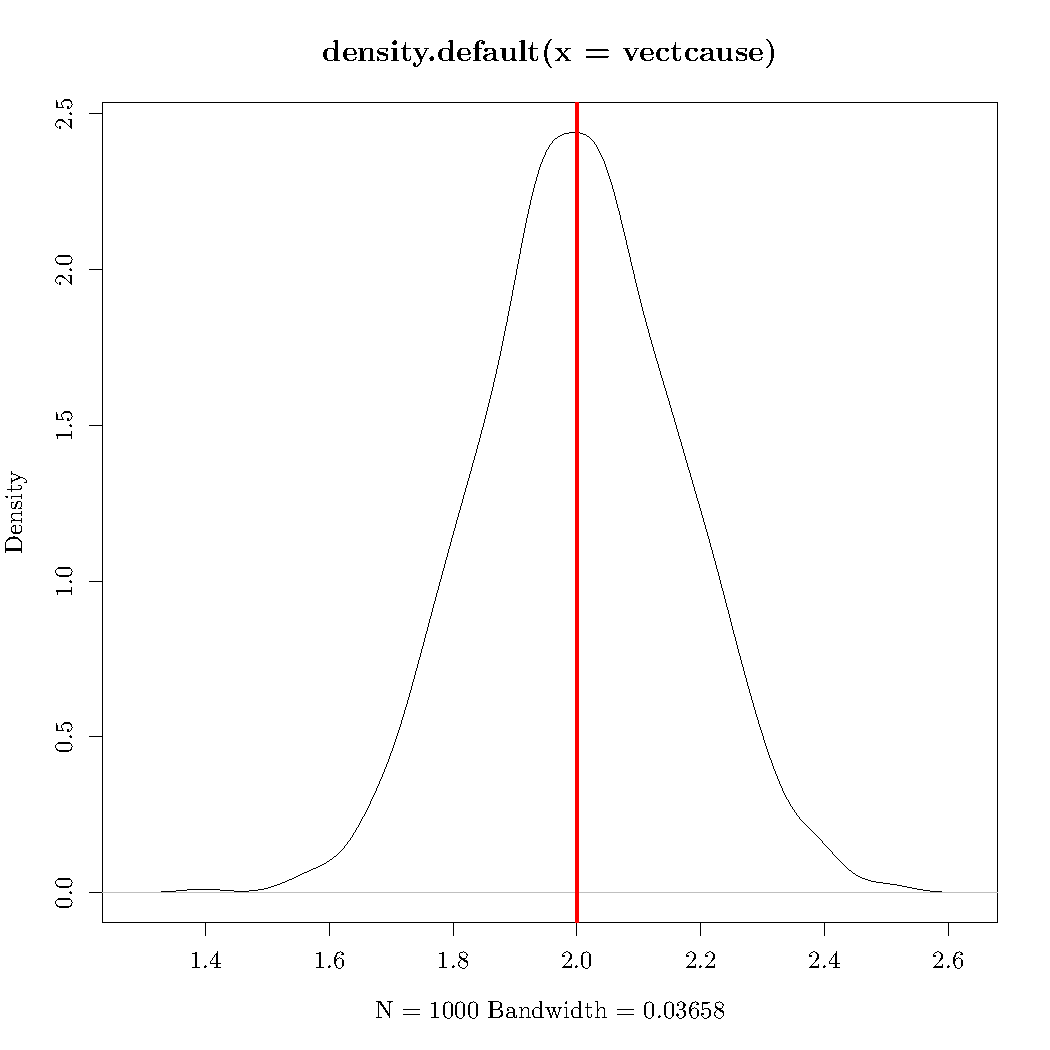
\includegraphics[width=0.6\textwidth]{figure/repmod-1} 

}


\begin{kframe}\begin{alltt}
\hlkwd{mean}\hlstd{(vectcause);}\hlkwd{sd}\hlstd{(vectcause)}\hlopt{/}\hlstd{(}\hlkwd{sqrt}\hlstd{(}\hlnum{1000}\hlstd{))}
\end{alltt}
\begin{verbatim}
## [1] 2.004635
## [1] 0.005116896
\end{verbatim}
\end{kframe}
\end{knitrout}
Which seems very reasonable.

However, the accuracy is lower. Interestingly, only the direct path estimation (the variance, on the slot ["cause";"cause"]) is blured by the correlation between the cause and the first consequence:
\begin{knitrout}
\definecolor{shadecolor}{rgb}{0.969, 0.969, 0.969}\color{fgcolor}\begin{kframe}
\begin{alltt}
\hlkwd{vcov}\hlstd{(m0)}
\end{alltt}
\begin{verbatim}
##               (Intercept)        cause consequence1
## (Intercept)   0.031624712  0.015386584 -0.005322435
## cause         0.015386584  0.009704506 -0.003112043
## consequence1 -0.005322435 -0.003112043  0.001044205
\end{verbatim}
\begin{alltt}
\hlkwd{vcov}\hlstd{(m1)}
\end{alltt}
\begin{verbatim}
##               (Intercept)        cause consequence1
## (Intercept)   0.031139826  0.042393309 -0.005362294
## cause         0.042393309  0.068504917 -0.008542076
## consequence1 -0.005362294 -0.008542076  0.001071723
\end{verbatim}
\end{kframe}
\end{knitrout}

Probably, modelling explicitly the causal path would help to deal with the loss of accuracy. 


I tried with a simple bayesian model. For some reasons, KnitR does not want to write this sink on the source folder so the model must be put by hand in a .txt file. 

\begin{knitrout}
\definecolor{shadecolor}{rgb}{0.969, 0.969, 0.969}\color{fgcolor}\begin{kframe}
\begin{alltt}
\hlkwd{library}\hlstd{(R2jags)}
\end{alltt}


{\ttfamily\noindent\itshape\color{messagecolor}{\#\# Loading required package: rjags\\\#\# Loading required package: coda\\\#\# Loading required package: lattice\\\#\# Linked to JAGS 3.4.0\\\#\# Loaded modules: basemod,bugs\\\#\# \\\#\# Attaching package: 'R2jags'\\\#\# \\\#\# The following object is masked from 'package:coda':\\\#\# \\\#\#\ \ \ \  traceplot}}\begin{alltt}
\hlcom{# }
\hlcom{# sink("simpleB.txt")}
\hlcom{# cat("}
\hlcom{#     model \{}
\hlcom{#     #priors and constraints}
\hlcom{#     AB~dunif(-10,10)}
\hlcom{#     AC~dunif(-10,10)}
\hlcom{#     BC~dunif(-10,10)}
\hlcom{#     intB~dunif(-10,10)}
\hlcom{#     intC~dunif(-10,10)}
\hlcom{#     tauB<-pow(sdB,-2)}
\hlcom{#     tauC<-pow(sdC,-2)}
\hlcom{#     sdB~dunif(0,10)}
\hlcom{#     sdC~dunif(0,10)}
\hlcom{#     #likelihood}
\hlcom{#     for (i in 1:S)    }
\hlcom{#       \{}
\hlcom{#         oB[i]~dnorm(B[i],tauB)}
\hlcom{#         B[i]<-intB+AB*oA[i]}
\hlcom{#         oC[i]~dnorm(C[i],tauC)}
\hlcom{#         C[i]<-intC+AC*oA[i]+BC*oB[i]}
\hlcom{#       \}}
\hlcom{# }
\hlcom{#     \}}
\hlcom{#     ",fill = TRUE)}
\hlcom{# sink()}
\end{alltt}
\end{kframe}
\end{knitrout}

If I run it for the first (not too correlated) data set:

\begin{knitrout}
\definecolor{shadecolor}{rgb}{0.969, 0.969, 0.969}\color{fgcolor}\begin{kframe}
\begin{alltt}
\hlstd{dataB}\hlkwb{<-}\hlkwd{list}\hlstd{(}\hlkwc{oB}\hlstd{=df}\hlopt{$}\hlstd{consequence1,}\hlkwc{oA}\hlstd{=df}\hlopt{$}\hlstd{cause,}\hlkwc{S}\hlstd{=}\hlkwd{nrow}\hlstd{(df),}\hlkwc{oC}\hlstd{=df}\hlopt{$}\hlstd{consequence2)}
\hlstd{initsB} \hlkwb{<-} \hlkwa{function}\hlstd{()} \hlkwd{list}\hlstd{(}\hlkwc{AB} \hlstd{=}\hlkwd{runif}\hlstd{(}\hlkwc{n}\hlstd{=}\hlnum{1}\hlstd{,}\hlopt{-}\hlnum{10}\hlstd{,}\hlnum{10}\hlstd{),}\hlkwc{AC}\hlstd{=}\hlkwd{runif}\hlstd{(}\hlkwc{n}\hlstd{=}\hlnum{1}\hlstd{,}\hlopt{-}\hlnum{10}\hlstd{,}\hlnum{10}\hlstd{),}\hlkwc{BC}\hlstd{=}\hlkwd{runif}\hlstd{(}\hlkwc{n}\hlstd{=}\hlnum{1}\hlstd{,}\hlopt{-}\hlnum{10}\hlstd{,}\hlnum{10}\hlstd{))}
\hlstd{paramsB} \hlkwb{<-} \hlkwd{c}\hlstd{(}\hlstr{"AB"}\hlstd{,}\hlstr{"AC"}\hlstd{,}\hlstr{"BC"}\hlstd{)}
\hlcom{# MCMC settings}
\hlstd{ni} \hlkwb{<-} \hlnum{5000} \hlstd{; nt} \hlkwb{<-} \hlnum{10} \hlstd{; nb} \hlkwb{<-} \hlnum{1000} \hlstd{; nc} \hlkwb{<-} \hlnum{3}
\hlstd{B1}\hlkwb{<-}\hlkwd{jags}\hlstd{(dataB,initsB,paramsB,}\hlstr{"simpleB.txt"}\hlstd{,}
         \hlkwc{n.chains} \hlstd{= nc,} \hlkwc{n.thin} \hlstd{= nt,} \hlkwc{n.iter} \hlstd{= ni,} \hlkwc{n.burnin} \hlstd{= nb,} \hlkwc{working.directory} \hlstd{=} \hlkwd{getwd}\hlstd{())}
\end{alltt}


{\ttfamily\noindent\itshape\color{messagecolor}{\#\# module glm loaded}}\begin{verbatim}
## Compiling model graph
##    Resolving undeclared variables
##    Allocating nodes
##    Graph Size: 8015
## 
## Initializing model
\end{verbatim}
\begin{alltt}
\hlkwd{print}\hlstd{(B1)}
\end{alltt}
\begin{verbatim}
## Inference for Bugs model at "simpleB.txt", fit using jags,
##  3 chains, each with 5000 iterations (first 1000 discarded), n.thin = 10
##  n.sims = 1200 iterations saved
##           mu.vect sd.vect     2.5%      25%      50%      75%    97.5%
## AB          2.980   0.020    2.942    2.967    2.979    2.994    3.020
## AC          2.044   0.105    1.843    1.970    2.049    2.119    2.250
## BC          3.969   0.035    3.902    3.946    3.968    3.994    4.036
## deviance 8393.553   3.731 8388.144 8390.806 8392.850 8395.766 8401.866
##           Rhat n.eff
## AB       1.001  1200
## AC       1.005   350
## BC       1.005   360
## deviance 1.000  1200
## 
## For each parameter, n.eff is a crude measure of effective sample size,
## and Rhat is the potential scale reduction factor (at convergence, Rhat=1).
## 
## DIC info (using the rule, pD = var(deviance)/2)
## pD = 7.0 and DIC = 8400.5
## DIC is an estimate of expected predictive error (lower deviance is better).
\end{verbatim}
\end{kframe}
\end{knitrout}

And now for the second (much more correlated) data set:
\begin{knitrout}
\definecolor{shadecolor}{rgb}{0.969, 0.969, 0.969}\color{fgcolor}\begin{kframe}
\begin{alltt}
\hlstd{dataB}\hlkwb{<-}\hlkwd{list}\hlstd{(}\hlkwc{oB}\hlstd{=df2}\hlopt{$}\hlstd{consequence1,}\hlkwc{oA}\hlstd{=df2}\hlopt{$}\hlstd{cause,}\hlkwc{S}\hlstd{=}\hlkwd{nrow}\hlstd{(df2),}\hlkwc{oC}\hlstd{=df2}\hlopt{$}\hlstd{consequence2)}
\hlstd{initsB} \hlkwb{<-} \hlkwa{function}\hlstd{()} \hlkwd{list}\hlstd{(}\hlkwc{AB} \hlstd{=}\hlkwd{runif}\hlstd{(}\hlkwc{n}\hlstd{=}\hlnum{1}\hlstd{,}\hlopt{-}\hlnum{10}\hlstd{,}\hlnum{10}\hlstd{),}\hlkwc{AC}\hlstd{=}\hlkwd{runif}\hlstd{(}\hlkwc{n}\hlstd{=}\hlnum{1}\hlstd{,}\hlopt{-}\hlnum{10}\hlstd{,}\hlnum{10}\hlstd{),}\hlkwc{BC}\hlstd{=}\hlkwd{runif}\hlstd{(}\hlkwc{n}\hlstd{=}\hlnum{1}\hlstd{,}\hlopt{-}\hlnum{10}\hlstd{,}\hlnum{10}\hlstd{))}
\hlstd{paramsB} \hlkwb{<-} \hlkwd{c}\hlstd{(}\hlstr{"AB"}\hlstd{,}\hlstr{"AC"}\hlstd{,}\hlstr{"BC"}\hlstd{)}
\hlcom{# MCMC settings}
\hlstd{ni} \hlkwb{<-} \hlnum{5000} \hlstd{; nt} \hlkwb{<-} \hlnum{10} \hlstd{; nb} \hlkwb{<-} \hlnum{1000} \hlstd{; nc} \hlkwb{<-} \hlnum{3}
\hlstd{B2}\hlkwb{<-}\hlkwd{jags}\hlstd{(dataB,initsB,paramsB,}\hlstr{"simpleB.txt"}\hlstd{,}
         \hlkwc{n.chains} \hlstd{= nc,} \hlkwc{n.thin} \hlstd{= nt,} \hlkwc{n.iter} \hlstd{= ni,} \hlkwc{n.burnin} \hlstd{= nb,} \hlkwc{working.directory} \hlstd{=} \hlkwd{getwd}\hlstd{())}
\end{alltt}
\begin{verbatim}
## Compiling model graph
##    Resolving undeclared variables
##    Allocating nodes
##    Graph Size: 8015
## 
## Initializing model
\end{verbatim}
\begin{alltt}
\hlkwd{print}\hlstd{(B2)}
\end{alltt}
\begin{verbatim}
## Inference for Bugs model at "simpleB.txt", fit using jags,
##  3 chains, each with 5000 iterations (first 1000 discarded), n.thin = 10
##  n.sims = 1200 iterations saved
##           mu.vect sd.vect     2.5%      25%      50%      75%    97.5%
## AB          7.970   0.020    7.932    7.956    7.969    7.983    8.009
## AC          2.322   0.241    1.844    2.187    2.323    2.468    2.856
## BC          3.960   0.030    3.895    3.942    3.960    3.977    4.020
## deviance 8395.541   3.822 8390.197 8392.721 8394.981 8397.561 8404.895
##           Rhat n.eff
## AB       1.004   470
## AC       1.091    37
## BC       1.107    34
## deviance 1.011   230
## 
## For each parameter, n.eff is a crude measure of effective sample size,
## and Rhat is the potential scale reduction factor (at convergence, Rhat=1).
## 
## DIC info (using the rule, pD = var(deviance)/2)
## pD = 7.3 and DIC = 8402.8
## DIC is an estimate of expected predictive error (lower deviance is better).
\end{verbatim}
\end{kframe}
\end{knitrout}

The uncertainty around AC is much larger in the second case... so it does not help.

hmmm, so there is nothing to do about this correlation between the causal paths?

\end{document}
